\documentclass[twoside]{article}
\usepackage{graphicx}
\usepackage{fancyhdr}
\pagestyle{fancy}
\fancyhead{} % clear all fields
\fancyhead[C]{\it {LCIO - Users manual}}
\fancyhead[RO,LE]{\thepage}
\fancyfoot{} % clear all fields
\renewcommand{\headrulewidth}{0pt}
\renewcommand{\footrulewidth}{0pt}
\renewcommand{\sfdefault}{phv}

%\setlength{\textheight}{235mm}
%\setlength{\textwidth}{145mm}
%\setlength{\topmargin}{-20mm}
%\setlength{\evensidemargin}{10mm}
%\setlength{\oddsidemargin}{10mm}
\setlength{\textheight}{235mm}
\setlength{\textwidth}{155mm}
\setlength{\topmargin}{-20mm}
\setlength{\evensidemargin}{10mm}
\setlength{\oddsidemargin}{10mm}

%\setlength{\parskip}{\baselineskip}
\setlength{\parindent}{0pt}

\bibliographystyle{apsrev}

\begin{document}

\title{LCIO [v00-07] -  Users manual}


\author{F. Gaede \\  DESY IT} 

\maketitle
\tableofcontents

\thispagestyle{fancy}
\section{INTRODUCTION \label{intro}}

LCIO is a persistency framework for the international linear collider detector 
simulation studies. It defines a data model, a user interface (API) and a file format.
It provides a C++ and a Java version with a common interface - a Fortran version is under 
development.

%(fig.~\ref{fig_motivation}).
%\begin{figure}
%\includegraphics[width=80mm]{motivation1.eps}
%\caption{Schematic overview of the simulation software chain. 
%LCIO defines a persistency framework for the simulation and reconstruction stages. 
%It is suited to replace the  plethora of different data and file formats currently 
%being used in linear collider simulation studies (denoted by the small arrows).
%\label{fig_motivation}}
%\end{figure}
This manual is intended for application developers that want to incorporate LCIO in their 
programs. This includes e.g. simulation developers as well as  physicists that want to 
read LCIO files for their analysis. It focuses on the practical aspects of using LCIO. A more 
general discussion can be found in \cite{lcio_chep} and other documents referred to at the 
LCIO homepage~\cite{lcio_home}.

\section{Installation}
\subsection{Getting LCIO}
If LCIO is not yet installed at your site you can get a recent copy from the CVS repository 
via anonymous checkout or download a tar-file with the source code from the LCIO 
homepage~\cite{lcio_home}. For the CVS checkout set the CVSROOT variable, e.g. on a Linux platform 
running {\it bash}:

\begin{verbatim}
  export CVSROOT=:pserver:anonymous@cvs.freehep.org:/cvs/lcio
\end{verbatim}

and then checkout a released version (see~\cite{lcio_home}), e.g.:
\begin{verbatim}
  mkdir lcio 
  cd lcio
  cvs co -d v00-07 -r v00-07 lcio
\end{verbatim}

\subsection{Requirements}
In order to build LCIO you need to have a Java VM (version 1.4 or higher) installed 
on your platform. This is true even if you only want to install the C++ version as the 
API-files are generated from an abstract description for Java and C++ using the 
AID~\cite{ref_aid} tool.
The C++ version of LCIO is developed under (Suse) Linux with gcc2.95.3 and tested
as well with gcc3.2, used on common RedHat distributions. 
As the -ansi switch is used it should be fairly easy to port it to other platforms, that have
an ANSI compliant C++ compiler installed, e.g. Windows/Cygwin.

\subsection {Building the library}
A few variables have to be set, e.g. on windows:
\begin{verbatim}
  set LCIO=c:\tony\projects\v00-06\lcio      <-- modify as appropriate
  set JDK_HOME=c:\java\j2sdk1.4.1            <-- modify as appropriate
  set PATH=%LCIO%\tools;%PATH%
\end{verbatim}
or using {\it bash}:
\begin{verbatim}
  cd v00-06
  export LCIO=$PWD
  export JDK_HOME=/usr/lib/j2sdk          <-- modify as appropriate
  export PATH=$LCIO/tools:$PATH
\end{verbatim}
%$ <- fixes syntax highlighting

To build the Java and C++ version simply type:
\begin{verbatim}
  ant
\end{verbatim}
 Or to do it step by step:
\begin{verbatim}
  ant aid.generate     <-- generates common API
  ant cpp              <-- creates C++
  ant aid              <-- creates Java  
\end{verbatim}

This will create the following libraries and executables:

\begin{verbatim}
 ./lib
      lcio.jar       <-- Java library (and executables)
      liblcio.a      <-- C++ library
 ./sio/lib
      libsio.a       <-- C++ version of sio 

 ./bin               <-- C++ examples and tools
      anajob
      copyfix
      dumpevent
      minijob
      recjob
      simjob
\end{verbatim}

To check whether the (C++) installation was successful run the {\it simjob} program:
\begin{verbatim}
  ./bin/simjob simjob.slcio
\end{verbatim}
This creates a simple LCIO file that you can read with 
\begin{verbatim}
  ./bin/anajob simjob.slcio
\end{verbatim}
The same for the Java version:
\begin{verbatim}
 ./bin/runSimJob.sh simjob.sclio
 ./bin/runAnalysisJob.sh simsob.sclio
\end{verbatim}


\section{Using LCIO}


\subsection{Java and C++ API} \label{sec_api}
Detailed documentation of the API is provided both for Java and C++, e.g. on the 
LCIO homepage~\cite{lcio_home} generated directly  from documentation in the source code using 
{\em javadoc} and {\em doxygen} respectively. 
If you are experienced in either Java or C++ you will probably 
find all you need to use LCIO in the corresponding version of the API documentation.
A few words on the design of LCIO might be helpful\ to browse the documentation.
LCIO is organized in a hierarchical package structure where the packages combine classes
with a well defined purpose as shown in table~\ref{tab_pkg}.  
\begin{table}
\begin{center}
\begin{tabular}{|c|c|p{6cm}|}
\hline
\rule[-5mm]{0mm}{10mm} C++ Namespace  &  Java package    &  Purpose \\ \hline \hline

 DATA  &  hep.lcio.data   &  The base interfaces of data entities.
 These interfaces are used to write the data, i.e. all user classes 
 that implement them can be made persistent with LCIO.\\ \hline
 EVENT  &  hep.lcio.event   & The base interfaces of the event.
 These interfaces extend the bare data interfaces with convenient 
 methods for analysis. They are used when LCIO events/data are read in. \\ \hline
 IO  &  hep.lcio.io   &  The base interfaces for io of data.\\ \hline
 IMPL  &  hep.lcio.implementation.event   & The default implementations of
 the base interfaces that are defined in EVENT. \\ \hline
 IOIMPL  &  hep.lcio.implementation.io   &  Extensions to the default implementations
 needed for IO. With the exception of LCFactory all other classes are for internal use only.\\ \hline
 SIO  &  hep.lcio.implementation.sio   & The persistency implementation using SIO.
 Users should not use any of the classes defined here explicitly but through their
 base interfaces defined in IO. \\ \hline
 LCIO  &   n.a. & The namespace lcio combines DATA, EVENT, IO and IMPL for user convenience
(\#include "lcio.h"). \\ \hline

\end{tabular}
\end{center}
\caption{Overview of the packages (namespaces) used in LCIO.}
\label{tab_pkg}
\end{table}
So a good starting point to browse the API documentation is the package/namespace overview.
Depending on the use case you will need mostly classes from one or two namespaces, e.g. if you need 
to read data from an existing LCIO file, you find most of the relevant classes in EVENT.
If you want to write data with LCIO you'll either need the implementation classes provided in IMPL
or implement the interface from DATA.

\begin{figure}
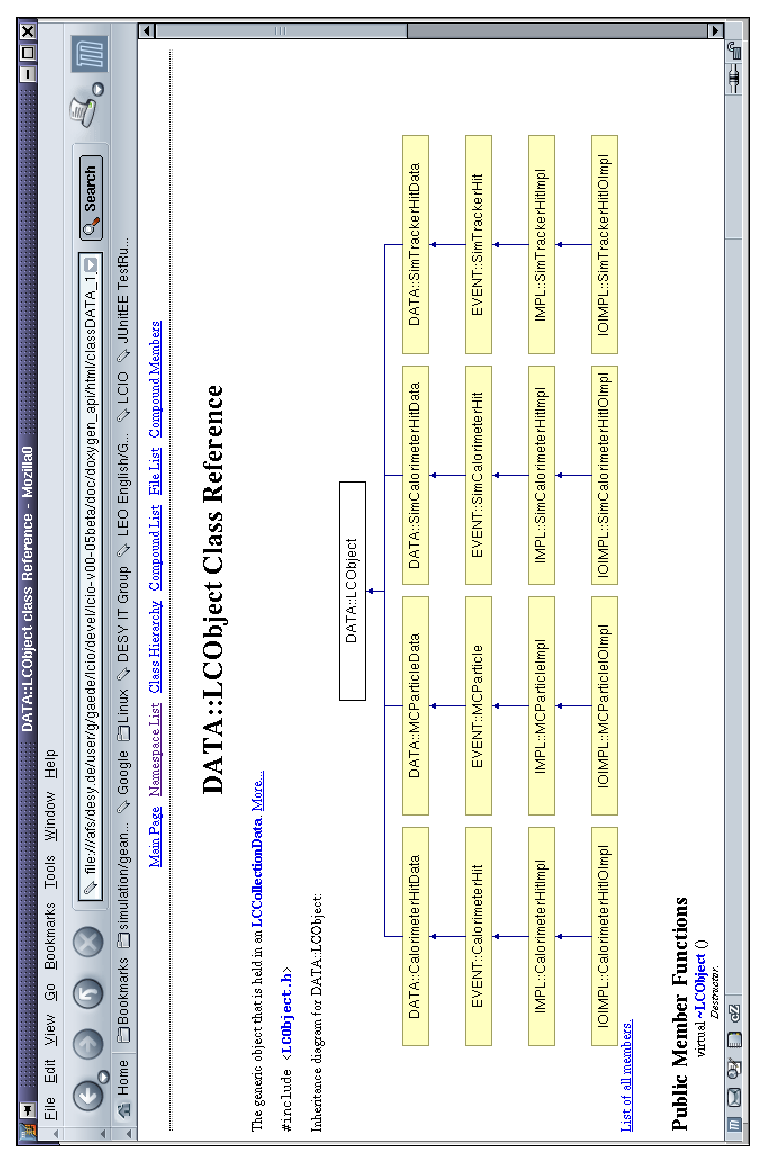
\includegraphics[width=95mm, angle=-90]{cpp_api.eps}
\caption{Documentation of the C++ API. The class description of {\em LCObject} gives you fast access 
to all data entities (classes). This class hierarchy also reflects the package hierarchy of LCIO.
\label{fig_cpp_api}}
\end{figure}


\subsection{Fortran API}
There will be a one to one mapping of the Fortran interface to the C++ API. For every class member 
function there will be a Fortran function with one additional integer parameter that holds the 
pointer to the underlying C++ object. This Fortran function is realized by a wrapper function 
that calls the underlying C++ implementation.
There is a naming convention, that allows to find the name of 
the wrapper function from the C++ name and vice versa. 


\subsection{Data model \label{sec_datamodel}}

Figure~\ref{fig_datamodel} shows the data entities that are currently defined by LCIO. 
\begin{figure}
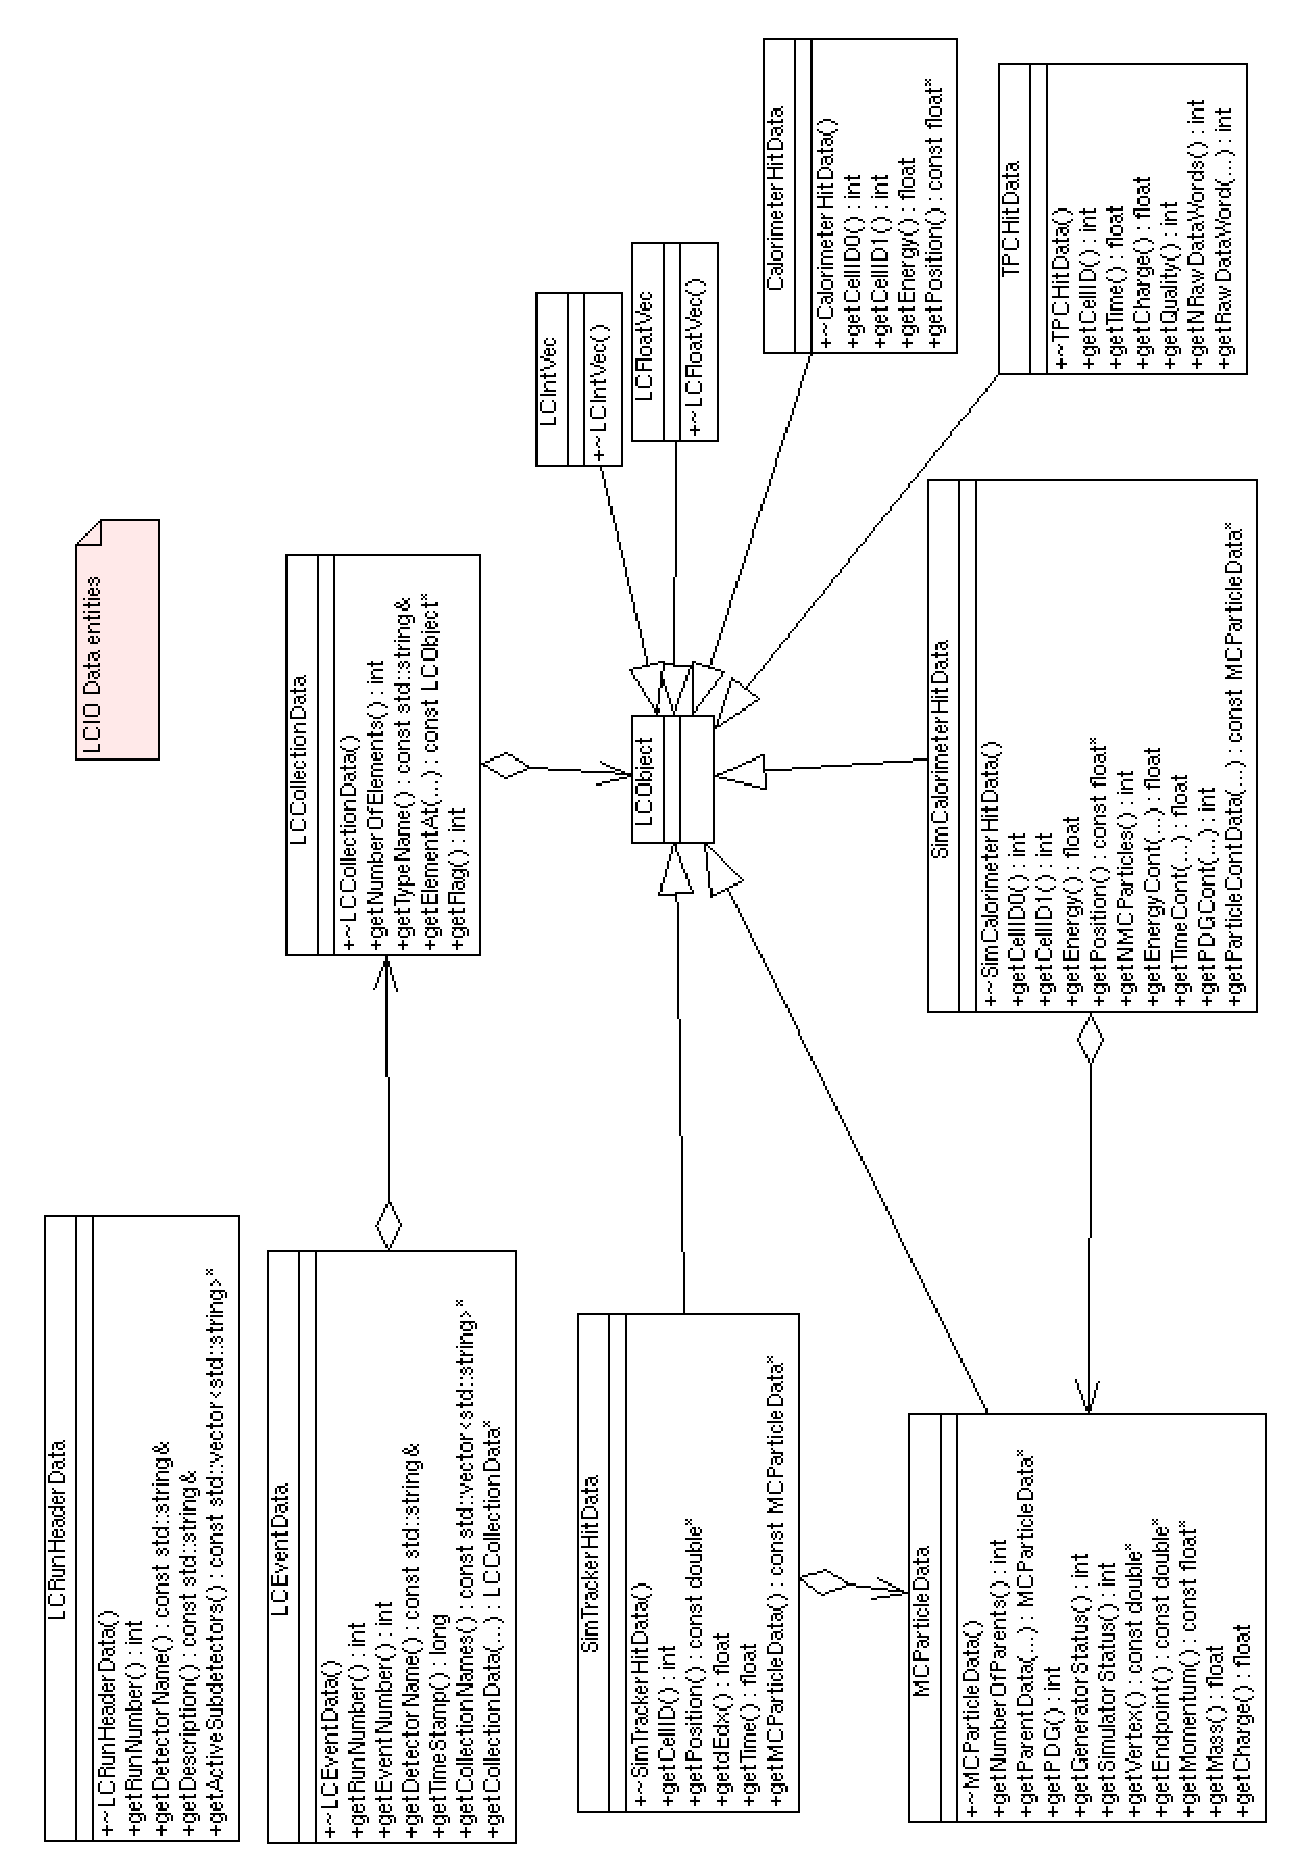
\includegraphics[width=150mm]{datamodel.eps}
\caption{Overview of the data model defined by LCIO (all classes in namespace DATA). 
The boxes correspond to separate
data entities (classes) and the arrows denote relationships between these entities.
The event data is stored in 'untyped' collections of LCObject subclasses. Every get-method
corresponds to a persistent attribute. 
Only the shown interface is used to write data, thus existing user classes can be made persistent 
by implementing this interface. 
\label{fig_datamodel}}
\end{figure}
Event data is stored in 'untyped' collections of LCObject subclasses. At the (full) simulation
output level the most important entities are the two generic hit classes {\em SimTrackerHit} and 
{\em SimCalorimeterHit}. Both classes have links to the generated particle ({\em MCParticle}) that 
contributed to the hit.
Users are free to store collections of {\em float} and {\em int} vectors/arrays of arbitrary size
as 'extensions' to the data model, see \ref{examples}.

\subsection{Data format \label{sec_sio}}

As a first concrete data format for LCIO we chose to use SIO (Serial Input Output).
SIO has been developed at SLAC and has been used successfully in the {\em hep.lcd}
framework. It is a serial data format that is based on XDR and thus machine 
independent. While being a sequential format it still offers some OO-features, in 
particular it allows to store and retrieve references and pointers within one record.
In addition SIO includes on the fly data compression using zlib.
LCIO files that use SIO, i.e. all current ones, have the extension {\em .slcio}.


%\subsection{Examples} \label{examples} 
%There are a number of examples in the {\em src} directory of LCIO that demonstrate
%the usage of LCIO. Here we give a step to step introduction to the most important features.

\subsection{How to read LCIO files}
There are a number of examples in the {\em src} directory -- 
some examples for reading and accessing data can be found in:
\begin{verbatim}
  src/cpp/src/EXAMPLE
    anajob.cc
    dumpevent.cc
    recjob.cc
  src/cpp/src/IMPL
    LCTOOLS.cc

  src/java/hep/lcio/example
    AnalysisJob.java
    RecJob.java
    LCTools.java
\end{verbatim}

%\vspace{\baselineskip}
%{\bf File handling}\\
\subsubsection{File handling} 
Before you can read from an LCIO file you have to create an instance of LCReader using LCFactory:

\begin{verbatim}
  LCReader* lcReader = LCFactory::getInstance()->createLCReader() ;
\end{verbatim}
or in Java:
\begin{verbatim}
  LCReader lcReader = LCFactory.getInstance().createLCReader();
\end{verbatim}

The factory pattern is used to hide  the concrete implementation of the data 
format~(see \ref{sec_sio}) from user code.

In LCIO we use the exception mechanism for error handling. Thus opening and closing a file
has to be done in a {\em try-catch} block:
\begin{verbatim}
  try{
    
    lcReader->open( "my_data.slcio" ) ;
    
    // .... here we can read sth. from the file 

    lcReader->close() ;
  }
  catch(IOException& e){
    cout << " io error : " << e.what() << endl ;
  }
\end{verbatim}
and again the same in Java:
\begin{verbatim}
  try{

    lcReader.open( "my_data.slcio" ) ;

    // ... do sth. ....

    lcReader.close() ;
  }
  catch(IOException e){
    System.out.println(" io error : " +  e.getMessage() ) ;
  }

\end{verbatim}
It is obviously straight forward to get the Java version of the code from the C++ one
%\footnote{Replacing every \verb$'->'$ and \verb$'::'$ with \verb$'.'$ and removing all 
%\verb$'*'$ and '\&' does most of what is needed. }, 
so we only give example code in C++ from now on.

%\vspace{\baselineskip}
%{\bf Reading from the file}\\
\subsubsection{Reading from the file}
There are two different ways of reading data from an LCIO file. One is via 
'readNext{\em Something}()' methods, where {\em Something} is either the next RunHeader or the next 
Event. This way the user has control over what is beeing read from the file. On the other hand you 
can only read one type of {\em records } at a time as you don't know the exact number of events for 
each run. A simple event loop looks like this: 

\begin{verbatim}
    LCEvent*  evt;
    while( (evt = lcReader->readNextEvent()) != 0 ) {
      
      LCTOOLS::dumpEvent( evt ) ;
      
      nEvents ++ ;
    }
\end{verbatim}

For small applications and data files this is a reasonable way of analyzing data.

The other way of reading LCIO data files is via a {\em Listener} (or {\em Observer}) pattern.
In this approach you have to write your own analysis module(s) which implements the 
{\em LCRunListener} and {\em LCEventListener} interface and register those with the {\em LCReader}.
When reading the data stream the corresponding registered modules are called depending on the type 
of the current record. 

By writing modules for distinct tasks, e.g. vertex track reconstruction, 
track finding, clustering algorithms etc. this already defines an application framework for 
reconstruction with the LCEvent as underlying data structure.

For example you can define one analysis module as run and event listener:

\begin{verbatim}
// class for processing run and event records
class MyAnalysis : public LCRunListener, public LCEventListener{
 
public:
   MyAnalysis() ;
  ~MyAnalysis() ;
 
  void analyze( const LCEvent * evt )  ;
  void analyze(const LCRunHeader* run) ;
 
  void update( LCEvent * evt ) { /* not needed */ ;}
  void update(LCRunHeader* run){ /* not needed */ ;}
  //...
};
\end{verbatim}

Here the {\em analyze} methods are used, as they provide {\em read only} access to the data. In a 
reconstruction job you would probably use the {\em update} methods.
One could for example create histograms for every run in \verb$analyze(const LCRunHeader* run)$
and then fill the histograms in \verb$analyze( const LCEvent * evt )$.

The corresponding event loop (in the main program) might then look something like this:

\begin{verbatim}
   MyAnalysis myAnalysis ;
   lcReader->registerLCRunListener( &myAnalysis ) ;
   lcReader->registerLCEventListener( &myAnalysis ) ;

   try{
     lcReader->readStream() ;
   }
   catch(IOException &e){
     cout<< " io error: " <<  e.what() << endl ;
   }
\end{verbatim}




%\vspace{\baselineskip}
%{\bf Accessing the data}\\
\subsubsection{Accessing the data}
Check the API documentation and the examples on how to access the data in the LCIO data structures.
Mostly this is straight forward, e.g. printing run data is as easy as:

\begin{verbatim}
  LCRunHeader *runHdr ;
  ...  
  cout << "  Run : " << runHdr->getRunNumber() 
       << " - "      << runHdr->getDetectorName() 
       << ":  "      << runHdr->getDescription()  
       << endl ;
\end{verbatim}

In order to access the information stored in the event, you need to know the collection names that 
hold the relevant data as well as the type of the objects, e.g. to access the TPC hits on could 
write code like the following:

\begin{verbatim}
  const LCCollection* col = evt->getCollection("TPCHits") ;

  int nHits =  col->getNumberOfElements() ;

  for( int i=0 ; i< nHits ; i++ ){

    const SimCalorimeterHit* hit = 
      dynamic_cast<const SimCalorimeterHit*>( col->getElementAt( i ) ) ;

      cout << "    hit " << i << " - energy: "  
           << hit->getEnergy() ;

    ...
  }
\end{verbatim}

A few comments are in order:
\begin{itemize}
\item{ {\bf collection name:} LCIO stores collections under user defined names. In order to retrieve 
the collection from the data, you need to know this name. Usually the person that created a data 
file will also have provided some documentation on the content (and on collection names). \\
NB: The underlying implementation of the LCIO data format is {\em self documenting}, i.e. information
on collection names and types is included in the files. This is used in the \verb$anajob$ and 
\verb$dumpevent$ example programs - run either of those to print collection names and 
types of an unknown LCIO file.
}

\item{ {\bf casts:} as LCIO uses 'untyped' collections, we have to up-cast from {\em LCObject} to 
the corresponding type, i.e. we need to know the type of the data. This is analogous to the 
{\em Collection} interface in Java. As C++ does not provide a common base class we had to 
introduce {\em LCObject} as a common base for event data in LCIO.
}

\item{ {\bf const pointer: } most methods in the C++ DATA interface (the {\em get}-methods) 
return a {\em const} pointer. This is to prevent from accidental modification of persistent data.
If you are  new to C++ -- const pointers are a bit cumbersome. Basically they don't allow you to call
any methods on the object pointed at, that are not declared const as well. \\
As Java does not have a similar concept we will probably remove const pointers from the C++
version in a future release.
}
\end {itemize}


\subsection{How to write LCIO files}

Some examples for writing data with LCIO can be found in
\begin{verbatim}
  src/cpp/src/EXAMPLE
    simjob.cc
    recjob.cc
  src/java/hep/lcio/example
    SimJob.java
    RecJob.java
\end{verbatim}

%\vspace{\baselineskip}
%{\bf File handling}\\
\subsubsection{File handling}
Before you can write to an LCIO file you have to create an instance of LCWriter using LCFactory:

\begin{verbatim}
  LCWriter* lcWriter = LCFactory::getInstance()->createLCWriter() ;
\end{verbatim}
or in Java:
\begin{verbatim}
  LCWriter lcWriter = LCFactory.getInstance().createLCWriter();
\end{verbatim}


Opening and closing the file is the same as described for the LCReader - include everything in a
{\em try-catch} block, e.g. in Java:
\begin{verbatim}
  try{

    lcWriter.open( "my_data.slcio" ) ;

    // ... write sth. to the file....

    lcWriter.close() ;
  }
  catch(IOException e){
    System.out.println(" io error : " +  e.getMessage() ) ;
  }
\end{verbatim}


%\vspace{\baselineskip}
%{\bf Writing to the file}\\
\subsubsection{Writing to the file}
As mentioned in section~\ref{sec_api} the LCWriter interface only uses the interfaces 
in DATA/hep.lcio.data. So all classes implementing these interfaces can be written with LCIO.
This can be used for existing classes in already existing applications. 
If  you design a new application in either Java or C++ you should consider to use the implementation
classes (IMPL/hep.lcio.implementation.event) that LCIO provides.
These are also used in the following examples. The principle steps involved are: 
create an instance of the implementation class, set the attributes and then call the corresponding
write method of the LCWriter interface.
For example writing the run header is done with:

\begin{verbatim}
   LCRunHeaderImpl* runHdr = new LCRunHeaderImpl ; 

   runHdr->setRunNumber( rn ) ;
   
   runHdr->setDetectorName( "HCALPPT" ) ;
   
   lcWrt->writeRunHeader( runHdr ) ;

   delete runHdr ;    // see below in  'LCIO Memory management in C++'
\end{verbatim}

The event works in the same way, except that we now also need collections - the necessary steps are:
create the event, set the event attributes, create a collection (with type name), add objects to the 
collection and finally add the collection to the event with a unique name:

\begin{verbatim}
  LCEventImpl*  evt = new LCEventImpl() ;     // create the event 

  evt->setRunNumber(  rn   ) ;
  evt->setEventNumber( i ) ;                  // set the event attributes

  LCCollectionVec* calVec = new LCCollectionVec( LCIO::SIMCALORIMETERHIT );   
                                              // create a collection for the 
                                              // type SimCalorimeterHit

  for(int j=0;j<NHITS;j++){
  
    SimCalorimeterHitImpl* hit = new SimCalorimeterHitImpl ;
    hit->setEnergy( 3.1415 )  ;
    //...  
    calVec->push_back( hit ) ;                // add hit objects to the collection
  }

  // ....
  evt->addCollection(calVec,"HCalPPTHits");   // add the collection with a name

  lcWrt->writeEvent( evt ) ;                  // write the event to the file


  // ------------ IMPORTANT ------------- ! 
  // we created the event so we need to delete it ...
  delete evt ;
  // -------------------------------------
\end{verbatim}

The last line is of course only relevant for C++:

%\vspace{\baselineskip}
%{\bf LCIO Memory management in C++}

\subsubsection{ LCIO Memory management in C++}
{\em The philosophy of memory management in LCIO is: " If you created the object (using new),
you are responsible for deleting it when it is no longer needed !".\\
In order to make this easier the LCEvent will delete everything that has been attached to the event.
If you are only reading, LCIO will create the objects and thus delete them (when reading the next 
object of the same type) -- thus no need for deleting on your side.\\
If you are reading and adding sth. to the event it is  LCIO that deletes the event 
(as it created it) and thus also everything attached to it -- again no need for deleting on your 
side.\\
As a rule of thumb: Use \verb$delete evt/runhdr$ at the end of every event/run loop where you 
created the event/runHeader and don't use delete in all other cases.\\
Of course if you use your own implementation of the DATA interface you are also responsible for the 
memory management.}
 

% Create the reference section using BibTeX:
%\bibliography{basename of .bib file}
\begin{thebibliography}{9}   % Use for  1-9  references
%\begin{thebibliography}{99} % Use for 10-99 references
\bibitem{lcio_chep}
 LCIO: A persistency framework for linear collider simulation studies. \\
{\footnotesize By Frank Gaede (DESY), Ties Behnke (DESY \& SLAC), Norman Graf, 
Tony Johnson (SLAC). SLAC-PUB-9992, CHEP-2003-TUKT001, Jun 2003. 5pp.
Talk given at 2003 Conference for Computing in High-Energy and Nuclear Physics (CHEP 03), 
La Jolla, California, 24-28 Mar 2003.
e-Print Archive: physics/0306114 / LC Note LC-TOOL-2003-053}
\bibitem{lcio_home}
LCIO Homepage: \\
{\footnotesize \verb#http://www-it.desy.de/physics/projects/simsoft/lcio/index.html#}


\end{thebibliography}


\end{document}

